% !TEX encoding = UTF-8
\documentclass[a4paper,twoside,11pt]{article}
\usepackage{ccs_physiqueIIPC}
\documents{\logicielpython,\textbf{2041JKPA.npy}}

	%ou - (rien), par défaut si on appelle pas la commande \documents
	%ou \film{avi}
	%ou \logiciel{Java}
	%ou \pdf{NOTICE} pour spécifier un doc du type 9999TEST-NOTICE.pdf
	%ou \doc pour ''Analyse de document''
\begin{document}
Dans le dispositif interférométrique représenté ci-dessous, la séparatrice $(S)$ est une lame semi-réfléchissante. 
\begin{center}
	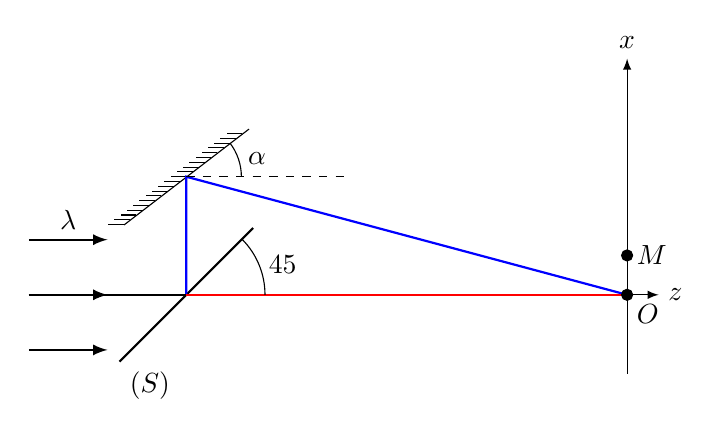
\begin{tikzpicture}
		\draw[thick] (45:-1.2)node[anchor=north west]{$(S)$}--(45:1.2);
		\draw[-latex] (-2,0)--(6,0)node[right]{$z$};
		\draw[-latex] ({1.5/tan(15)},-1)--++(0,4)node[above]{$x$};
		\draw (0,1.5)++(37.2:1)--++(37.5:-2);
		\foreach \x in {-1,-.9,...,1}
		{
			\draw (0,1.5)++(37.5:\x)--++(-.2,0);
		}
		\draw[thick,blue] (0,0)--(0,1.5)--++(-15:{1.5/sin(15)});
		\draw[thick,red] (0,0)--({1.5/tan(15)},0);
		\draw[fill] ({1.5/tan(15)},0)node[anchor=north west]{$O$}circle(2pt) ({1.5/tan(15)},.5)node[right]{$M$}circle(2pt);
		\draw[thick] (-2,0)--(0,0);
		\draw[thick,-latex] (-2,-.7)--++(1,0);
		\draw[thick,-latex] (-2,0)--++(1,0);
		\draw[thick,-latex] (-2,.7)--node[above]{$\lambda$}++(1,0);
		\draw (1,0)arc[start angle=0,end angle=45,radius=1cm]node[right,pos=.5]{$\SI{45}{\degree}$};
		\draw[dashed] (0,1.5)--++(2,0);
		\draw (.7,1.5)arc[start angle=0,end angle=37.7,radius=.7cm]node[right,pos=.5]{$\alpha$};
	\end{tikzpicture}
\end{center}
Le système est éclairé par un faisceau parallèle de lumière	monochromatique (de longueur d'onde ${\lambda=\SI{.6}{\um}}$). 

On note $A_0$ l'amplitude en $O$ du rayon ayant traversé la séparatrice, et $A_1$ celle du rayon réfléchi sur le miroir.
L'angle $\alpha$ est très proche de $\SI{45}{\degree}$, et on pourra poser $2\alpha=\dfrac{\pi}{2}-\varepsilon$ avec $\varepsilon\ll1$

\qt On suppose que  l'origine $O$ est choisie de telle façon que les
deux ondes y aient la même phase. Montrer que l'intensité lumineuse en $M(x, y, 0)$ peut s'écrire~:
$$
I=C_1+C_2\cos(Kx)
$$
où l'on précisera la valeur prise par $K$, $C_1$ et $C_2$ en fonction des paramètres du problème.
\qt Calculer l'interfrange en fonction de $\lambda$ et $\varepsilon$.
On définit le contraste par 
$$C=\dfrac{I_{max}-I_{min}}{I_{max}+I_{min}}$$
\qt Calculer le contraste des franges en fonction du rapport $r = A_1/A_0$. Comment choisir $r$ pour avoir contraste maximal ?


Le système précédent sert à éclairer un milieu qui contient des molécules porteuses d'un marqueur fluorescent.  On suppose que lorsque de telles molécules sont éclairées, une quantité proportionnelle à l'éclairement reçu devient fluorescente, on a donc une densité de molécules fluorescentes qui s'écrit $n(M)=KI(M)$ où $I$ est l'éclairement au point $M$. On note $D$ le coefficient de diffusion des molécules dans le milieu.

\qt Exprimer la densité de molécules fluorescentes après traitement par le système interférométrique. Comment va évoluer qualitativement, le profil $n(x,t)$ ?
\qt Donner l'équation  vérifiée par $n(x,t)$.\\
On cherche la solution de l'équation précédente sous la forme~:
$$
n(x,t)=n_0+f(x)\cdot  g(t)\quad \text{avec $g(t)=1$}
$$
\qt Préciser la forme de $n_0$ et $f(x)$. En déduire la forme de $g(t)$.\\

Pour simplifier, on suppose que chaque molécule fluorescente émet une intensité constante au cours du temps.

\qt Proposer un protocole expérimental permettant de mesurer $D$.
\info{Étude}{On fournit dans un script Python, pour des valeurs de $\varepsilon$ comprises entre \SI{.5}{\degree} et \SI{5}{\degree}, le graphe de $g(t)$.  L'utilisation des données est détaillée dans le script.
}
\qt Mettre en \oe uvre une méthode informatique permettant de déterminer $D$ à l'aide des données expérimentales. 
\end{document}
